%\begin{figure}[h]
%    \centering
%    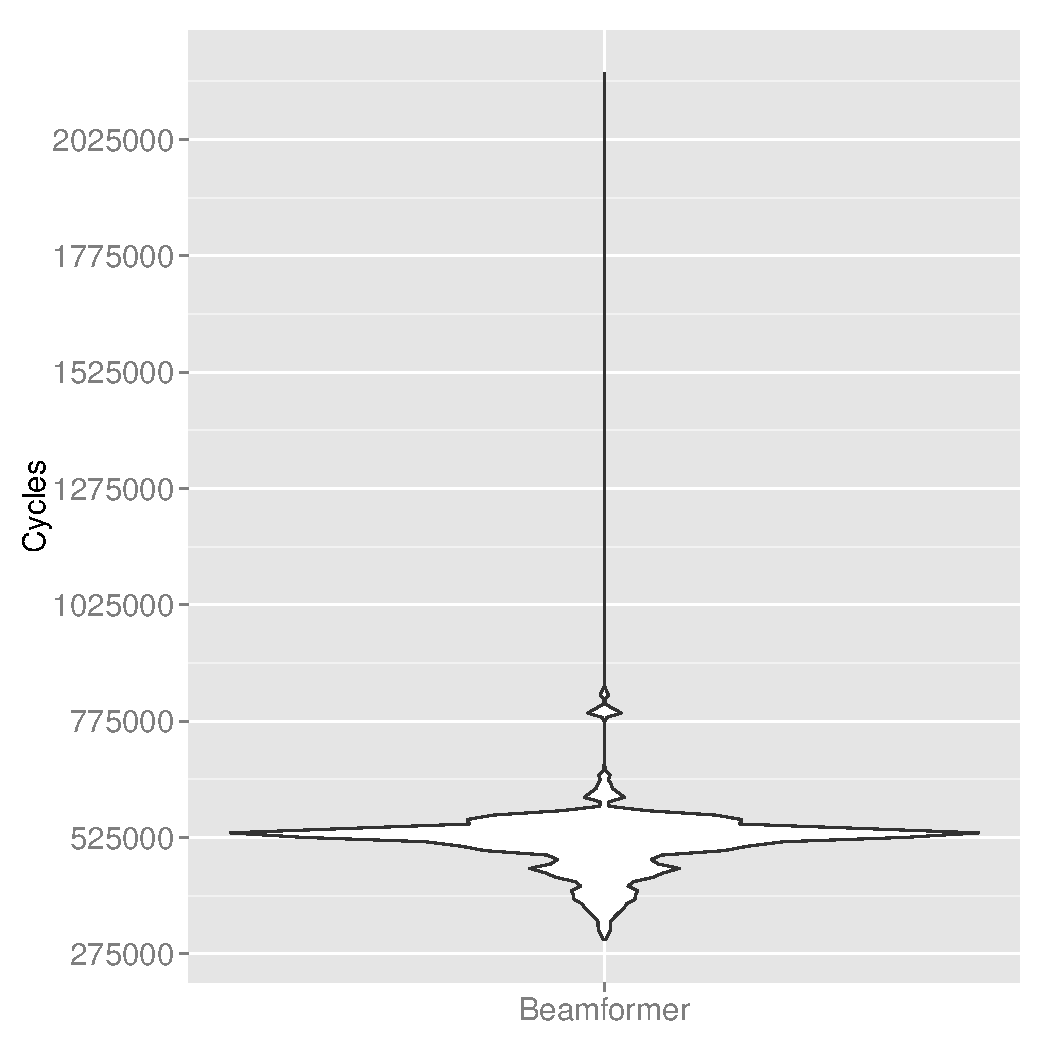
\includegraphics[width=0.7\textwidth]{streamit-paper/graphics/beamformer_motivation.pdf}
%    \caption{Distribution of the runtime for Beamformer resulting from an exhaustively exploration of the hardware/software co-design space.
%     The application has been partitioned into different number of threads and core compositions.}
%     \label{fig:beamformermotiv}
%\end{figure}

\begin{figure}[t]
    \centering
    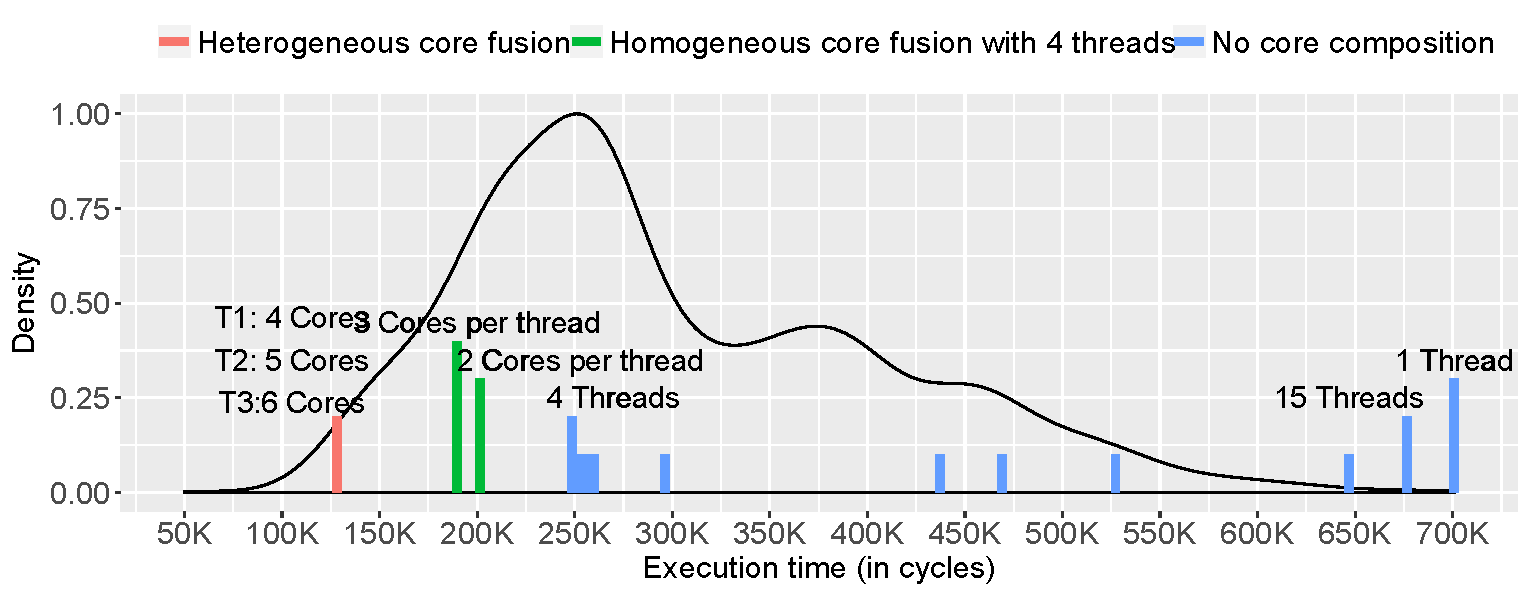
\includegraphics[width=1\textwidth]{streamit-paper/graphics/filterbank_motivation_2.pdf}
    \caption{Distribution of the runtime for FilterBank with different core composition and thread pairings. The dots on the X-axis represent specific configurations and their cycle counts.}
     \label{fig:threadcoremotiv}
\end{figure}

This section motivates the difficulty of finding a good mixture of thread partitioning and core allocation.
First, a simple experiment is conducted where the \bench{FilterBank} StreamIt benchmark is analysed.
The benchmark's tasks are partitioned into threads and a various number of cores are allocated to each thread.
The program is executed on a 16 core system.
Since one of the thread is a master thread which creates and joins all worker threads, this means that the benchmark can be partitioned in up to 15 threads.
As each thread must have at least one core assigned to, and not all cores have to be composed, the total number of configurations are:

\begin{equation}
15 + \sum_{n=2}^{15} \sum_{m=n}^{15} \frac{(m-1)!}{(n-1)!((m-1)-(n-1))!}
\label{eq:comb}
\end{equation}

In Equation~\ref{eq:comb}, the 15 represents the 15 different number of cores that can be composed for the single threaded version.
Thus there are 32767 combinations (exhaustive space) of thread mappings and core compositions pairings is generated.
Each design point is executed on the dynamic multicore simulator, the exact details about the experimental setup are presented later in section~\ref{sec:setup}.

Figure~\ref{fig:threadcoremotiv} presents the distribution of execution time, displayed as a cycle count, from a subset of the co-design space of \bench{FilterBank} as a density graph.
For this Figure, 1316 different thread/core combinations were explored, the reason this number was chosen will be explained later on in section~\ref{sec:setup}.
First, as can be seen in Figure~\ref{fig:threadcoremotiv}, the majority of the different combinations are found at around 250K cycles.
The worst point for \bench{FilterBank} can be found at the single core execution, which is a single core, single thread, resulting in an execution time of about 700K cycles, which is over 2x slower than the average case.
It is important to note that as the execution times get faster, the number of points grows smaller.
For the best execution points, which are far fewer than the average case (4x smaller density than the average case) the execution time can be as small as 125K cycles, which is 2x faster than the average case and 4x faster than the single core version.
Thus, if a good configuration is found, this can yield an important speedup compared to the average configuration.
However, the number of good configurations is low, this underlines the notion that finding a combination of threads and cores is a non-trivial endeavour, as randomly choosing a configuration will result in a suboptimal performance.
Indeed, whilst the average case is 2x faster than a single core, Figure~\ref{fig:threadcoremotiv} shows that there exists a good number of configurations that can lead to execution times that are slower than average case.

%Insert an example to show that it's a mix of threads and cores that matters.
Whilst there exists a large variety of thread-core combinations, certain design choices can be used to try and minimize the space.
For example, choosing to only do multithreading reduces the search space to 15 possible solutions whilst only combinations that lead to homogeneous core compositions reduces the search space to:
\begin{equation}
\sum_{n=1}^{15} \lfloor\frac{15}{n}\rfloor
\end{equation}
which is 45 possible solutions.
However, reducing the search space will limit the potential obtainable speedup.
Figure~\ref{fig:threadcoremotiv} also shows the performance distribution of different core-thread pairings.
Their location on the X-axis represents the execution time for that specific configuration.
The points represent a set of different design choices such as only using multithreading, using homogeneous core-compositions with threads and using heterogeneous core-compositions with threads.

As can be seen, using only multithreading can lead to some performance improvements, however it will not result in the optimal performance.
For the \bench{FilterBank} benchmark, 4 threads leads to the fastest execution time when only using multithreading.
This performance is in the highest peak of the density curve, which means that finding the best number of threads for the benchmark will only lead to an average performance in this case.
However, using too many threads, for example 15 threads, can lead to a degredaded performance compared to the average.
In this case, 15 threads is not much faster than using a single thread.
This is due to the fact that the communication overhead between threads will be too high compared to the actual computation of the benchmark.

Using the optimal number of threads, which is the number of threads that leads to the fastest execution time without core-composition as a baseline, homogeneous core-composition can then be explored.
In this case only 2 homogeneous pairings exist: 2 cores fused for each of the 4 threads or 3 cores fused for each of the 4 threads.
Figure~\ref{fig:threadcoremotiv} shows that homogeneous core-composition will outperform only using multithreading by 1.3x, however it is not the optimal solution.
In the end, using a heterogeneous configuration leads to a 1.5x speedup compared to the fastest homomgeneous configuration.
It's also important to note that the best heterogeneous core-composition required a different number of threads than the optimal number of threads previously describe.
Whilst this is the case in this example, section~\ref{sec:streamit:dse} will show that the optimal number of threads with and without core-composition are often the same or plus or minus one.
Therefore, it is important to consider all possible configurations to ensure the possibility of obtaining the best performance.

Figure~\ref{fig:threadcoremotiv} demonstrates that of the three scenarios that are explored, the heterogeneous core-composition with multiple threads is the optimal solution.
This means that the total space has to be explored in order to ensure that the fastest execution time can be found.
Due to the size of the space and the fact that there can be no apriori about good configurations, machine learning can be used to predict good configurations.
By exploring the space with a set of StreamIt benchmarks using different configurations for the processor, a machine learning model can learn what features correlate with the correct configuration.

These two examples illustrates the necessity for designing the technique to predict both the optimal number of threads and core composition to use.
The next section will present a more in-depth analysis of the design space before presenting our machine-learning predictive model.

